\section{Single Page application}
\label{sec:signle_page_application}
Single-page application (SPA) is a web application or web site that fits on a single web page with the goal of providing a more fluid user experience akin to a desktop application. In a SPA, either all necessary code – HTML, JavaScript, and CSS – is retrieved with a single page load,[31] or the appropriate resources are dynamically loaded and added to the page as necessary, usually in response to user actions. The page does not reload at any point in the process, nor does control transfer to another page, although modern web technologies (such as those included in the HTML5 pushState() API) can provide the perception and navigability of separate logical pages in the application. Interaction with the single page application often involves dynamic communication with the web server behind the scenes.
\newline
SPAs use AJAX and HTML5 to create fluid and responsive Web apps, without constant page reloads. However, this means much of the work hap- pens on the client side, in JavaScript. For the traditional ASP.NET developer, it can be difficult to make the leap. Luckily, there are many open source JavaScript frameworks that make it easier to create SPAs.
In a traditional Web app, every time the app calls the server, the server renders a new HTML page. This triggers a page refresh in the browser.
\begin{figure}[htb]
 \centering
 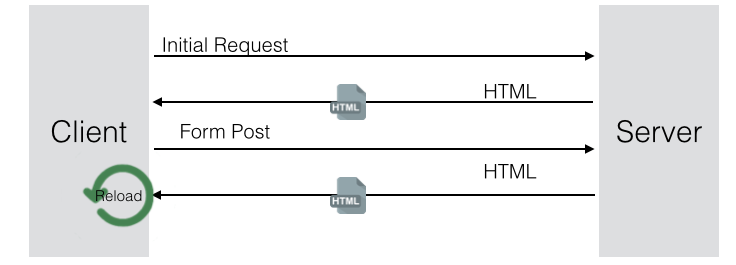
\includegraphics[width=1.0\linewidth]{images/chapter3/trad_life.png}\hfill
 \caption[Traditional Page Lifecycle]{The Traditional Page Lifecycle}
 \label{fig:traditional_page_lifecycle}
\end{figure}
In an SPA, after the first page loads, all interaction with the server happens through AJAX calls. These AJAX calls return data - not markup - usually in JSON format. The app uses the JSON data to update the page dynamically, without reloading the page.
One benefit of SPAs is obvious: Applications are more fluid and responsive, without the jarring effect of reloading and re-rendering the page.
\begin{figure}[htb]
 \centering
 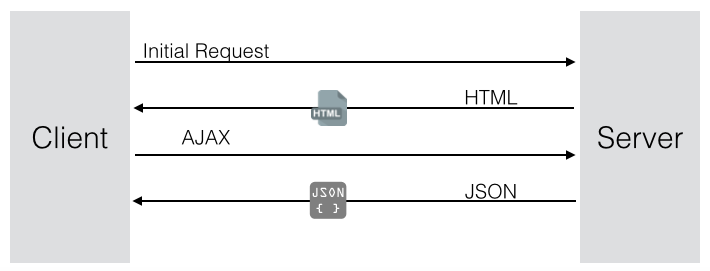
\includegraphics[width=1.0\linewidth]{images/chapter3/spa_life.png}\hfill
 \caption[SPA Lifecycle]{The SPA Lifecycle}
 \label{fig:spa_lifecycle}
\end{figure}